\begin{frame}{Sum of Orbit Cosines is Conserved!}
\begin{equation*}
\sum_{i=1}^{3}{\cos\theta_i}=1+\frac{r}{R}=\gamma{L}-3
\end{equation*}

\begin{figure}
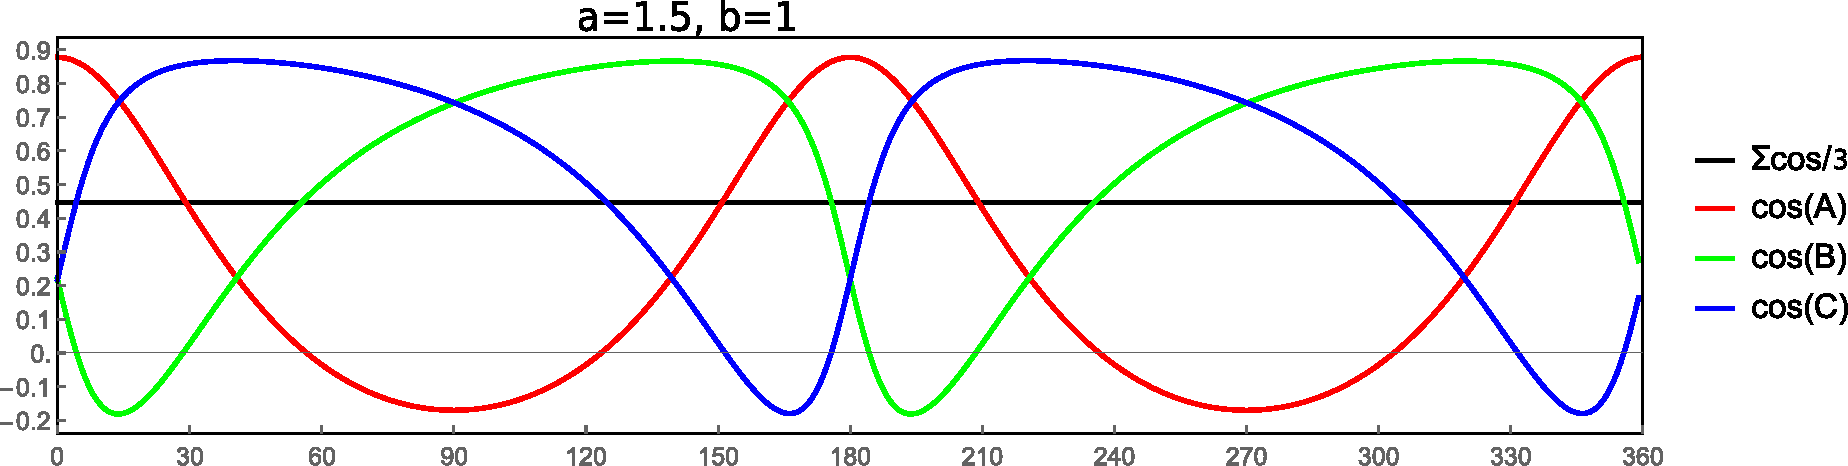
\includegraphics[width=.8\textwidth]{pics/0090_cosine_sum_n3.pdf}
\end{figure}
\end{frame}

\begin{frame}{Product of Excentral Cosines is Conserved!  \href{https://youtu.be/P8ykpE_ZbZ8}{[video]}}
\begin{tabular}{rl}
\begin{tabular}{r}
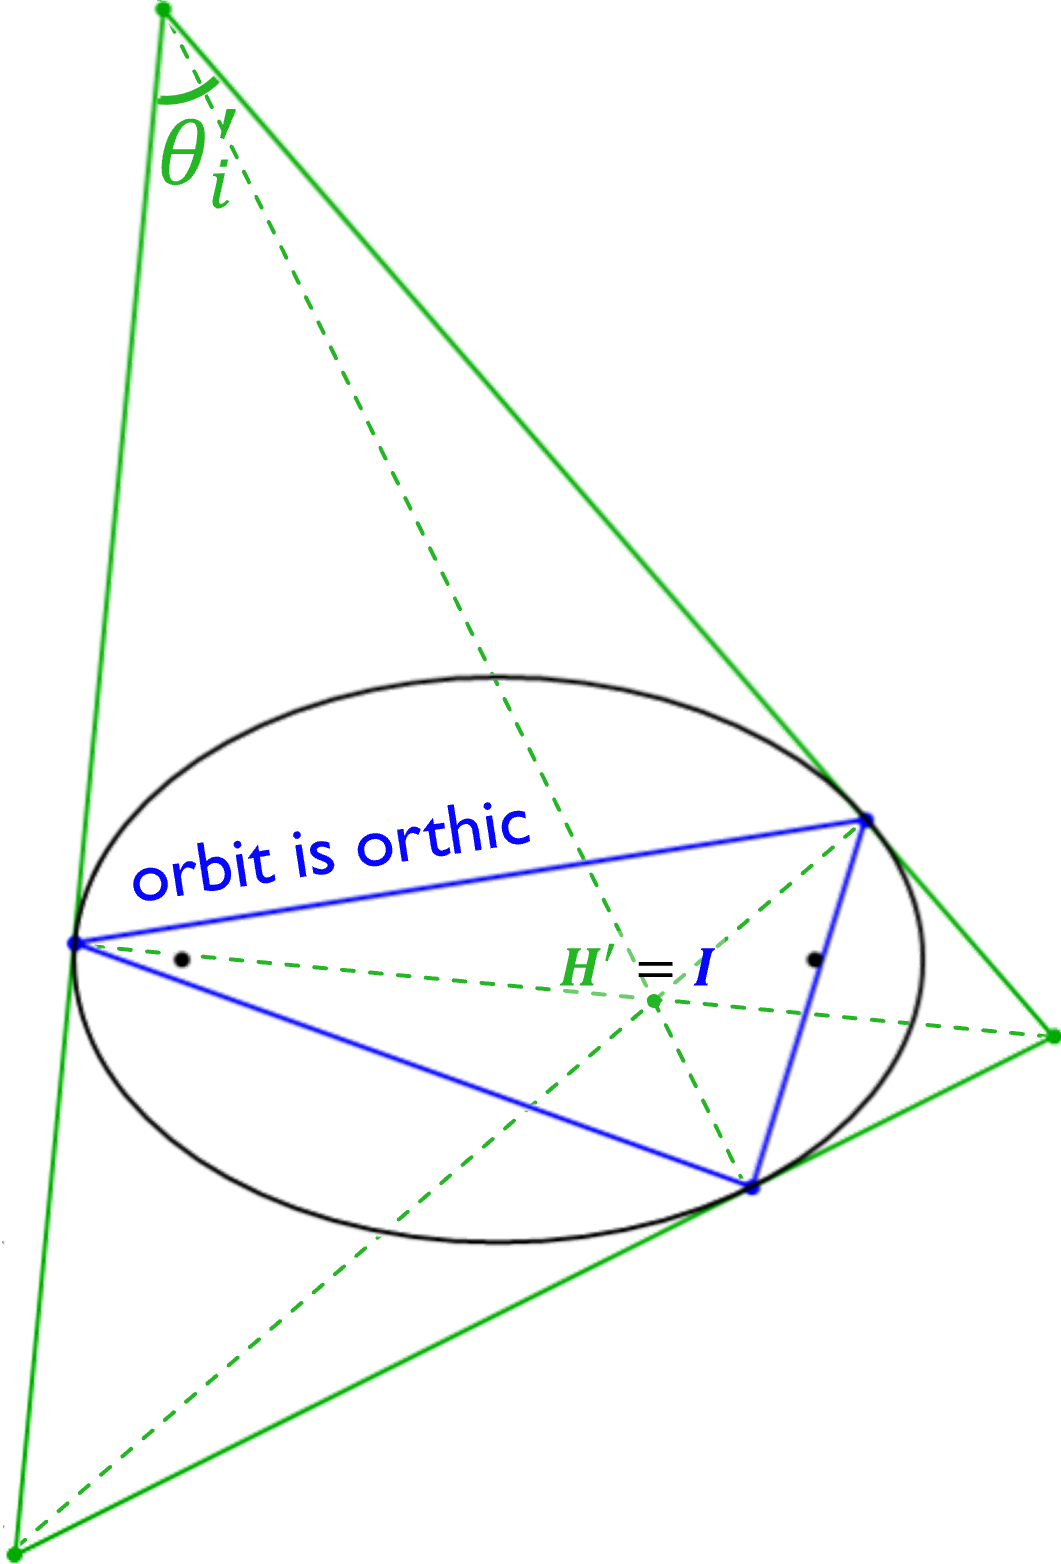
\includegraphics[height=.7\textheight]{pics/0076_product_of_excentral.png}
\end{tabular} & \begin{tabular}{l}
\parbox{0.5\linewidth}{
  \begin{minipage}{0.45\textwidth} $$\prod_{i=1}^{3}{|\cos\theta_i'|}=\frac{1}{4}\frac{r_h}{R_h}=\frac{\gamma{L}}{4}-1$$ \end{minipage}}
\end{tabular}  \\
\end{tabular}
\end{frame}

\begin{frame}{Orbit-to-Excentral Area Ratio is Conserved!}
\begin{tabular}{rl}
\begin{tabular}{r}
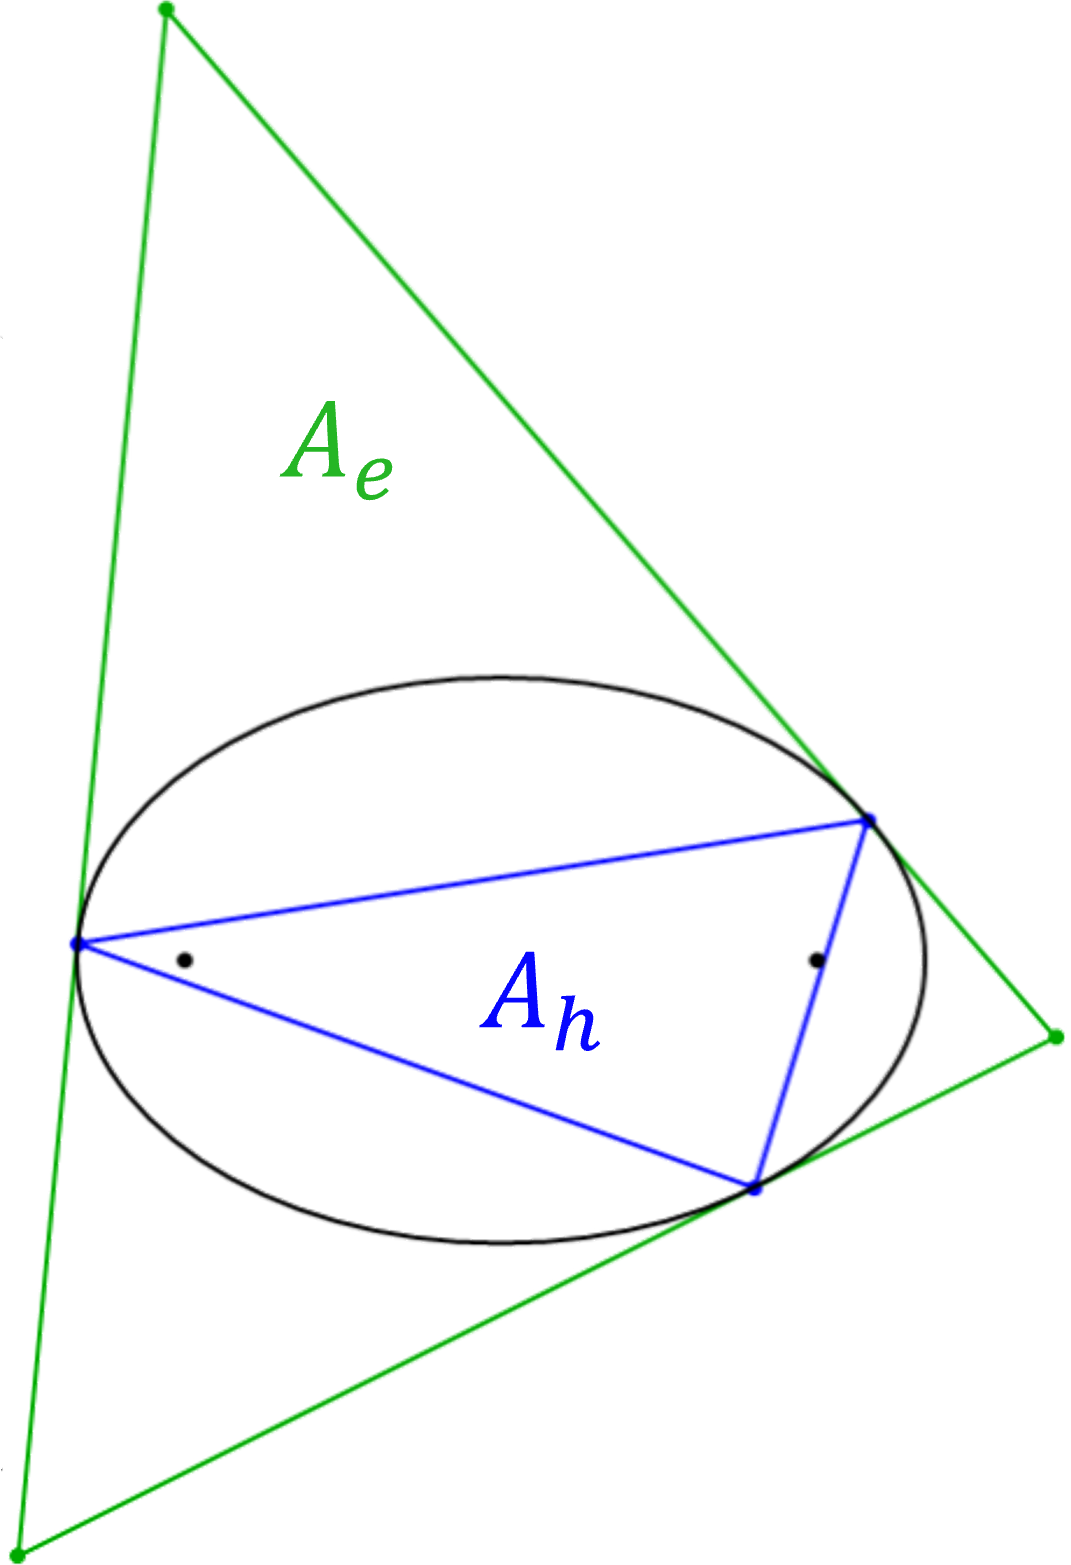
\includegraphics[height=.7\textheight]{pics/0077_area_ratio.png}
\end{tabular} & \begin{tabular}{l}
\parbox{0.5\linewidth}{
  \begin{minipage}{0.45\textwidth} $$\frac{A_h}{A_e}=\frac{1}{2}\frac{r_h}{R_h}$$ \end{minipage}}
\end{tabular}  \\
\end{tabular}
\end{frame}